\documentclass[a4paper, 12pt]{article}

\usepackage[T2A]{fontenc}
\usepackage[utf8]{inputenc}
\usepackage[english, russian]{babel}
\usepackage{amsmath}
\usepackage{graphicx}
\usepackage{subcaption}
\usepackage{float}
\usepackage{tabularx}
\usepackage{amsmath,booktabs}
\usepackage{array}
\righthyphenmin=2
\usepackage[left=20mm, top=15mm, right=15mm, bottom=15mm, nohead, footskip=10mm]{geometry} % настройки полей документа
\usepackage{caption}

%%%%%%%%%%%%CAPTION%%%%%%%
\DeclareCaptionLabelSeparator{dash}{ – }
\captionsetup{justification=centering,labelsep=dash}
\newcommand\tline[2]{$\underset{\text{#1}}{\text{\underline{\hspace{#2}}}}$}
\captionsetup[table]{justification=raggedright,singlelinecheck=off}
%%%%%%%TABLE%%%%
\renewcommand{\arraystretch}{1.8}
\renewcommand{\tabcolsep}{1cm}

%%%%%%%%%%%%%%%%%%%%%%%%%%%%%%%%%%
\begin{document} 
	
		\begin{titlepage}
		\centering
		{\fontsize{12pt}{5cm}\selectfont \bfseries Министерство образования и науки Российской Федерации} \\ \vspace{0.5cm}
		{\fontsize{7pt}{5cm}\selectfont ФЕДЕРАЛЬНОЕ ГОСУДАРСТВЕННОЕ АВТОНОМНОЕ ОБРАЗОВАТЕЛЬНОЕ УЧРЕЖДЕНИЕ ВЫСШЕГО ПРОФЕССИОНАЛЬНОГО ОБРАЗОВАНИЯ} \\ 
		\vspace{1cm}
		{\fontsize{12pt}{5cm}\selectfont \bfseries САНКТ-ПЕТЕРБУРГСКИЙ УНИВЕРСИТЕТ ИНФОРМАЦИОННЫХ ТЕХНОЛОГИЙ, МЕХАНИКИ И ОПТИКИ} \\ \vspace{1.5cm}
		
		{\fontsize{14pt}{5cm}\selectfont Кафедра \hspace{1cm} \underline{Систем Управления и Информатики}  \hspace{1cm} Группа \underline{Р3340}} \\ 
		\vspace{2cm}
		
		{\fontsize{20pt}{5cm}\selectfont \bfseries Лабораторная работа №9} \\
		{\fontsize{20pt}{5cm}\selectfont \bfseries “Экспериментальное построение частотных характеристик типовых динамических звеньев”} \\
		{\fontsize{14pt}{5cm}\selectfont Вариант - 02} \\
		\vspace{1.5cm}
		
		\flushleft
		
		{Выполнил \hspace{0.5cm} \tline{(фамилия, и.о.)}{10cm} (подпись)} \\
		\vspace{2cm}
		
		{Проверил \hspace{0.5cm} \tline{(фамилия, и.о.)}{10cm} (подпись)} \\
		\vspace{5cm}
		
		"\underline{\hspace{0.4cm}}"\hspace{0.1cm}\underline{\hspace{1.5cm}}\hspace{0.1cm}20\underline{\hspace{0.4cm}}г. \hspace{2cm} Санкт-Петербург, \hspace{2cm} 20\underline{\hspace{0.4cm}}г. \\ \vspace{1cm}
		
		Работа выполнена с оценкой \hspace{0.5cm} \underline{\hspace{10cm}} \\ 
		\vspace{1cm}
		Дата защиты "\underline{\hspace{0.4cm}}"\hspace{0.1cm}\underline{\hspace{1.5cm}}\hspace{0.1cm}20\underline{\hspace{0.4cm}}г.
		
	\end{titlepage}

\section*{Цель работы}
Изучение частотных характеристик типовых динамических звеньев и способов их построения.

\section*{Исходные данные}
В таблице 1 и 2 приведены исходные данные динамических звеньев 

\begin{table}[h!]
	\caption{Исходные данные}
	\label{data1}
	\begin{tabular}{|c|c|}
		\hline
		Тип звена & Передаточная функция\\
		\hline
		Колебательное & $\frac{k}{T^2s^2 + 2\xi Ts + 1}$\\
		\hline
		Идеальное интегрирующее & $\frac{k}{s}$\\
		\hline
		Изодромное & $\frac{k(1+Ts)}{s}$\\
		\hline
	\end{tabular}
\end{table}

\begin{table}[h!]

	\label{data2}
	\caption{Параметры}
	\begin{tabular}{|c|c|c|}
		\hline
		$k$ & $T$ & $\xi$ \\
		\hline
		2 & 0.5 & 0.15\\
		\hline
	\end{tabular}

\end{table}
		
\newpage		
		
\begin{center}
	\section{Колебательное звено}
\end{center}\par

В таблице \ref{tab:coleb} представлены экспериментальные данные колебательного звена.
Уравнение асимптотической ЛАЧХ
\begin{equation}
	L(\omega) = \begin{cases}
					20\lg(k), & \mbox{при } \omega<\omega_1;\\
					20\lg(k)-40\lg(T*\omega), & \mbox{при } \omega \geq \omega_1\\
					\omega = \frac{1}{T}
				\end{cases}
\end{equation}
		
\begin{table}[h]
	\caption{Экспериментальные данные колебательного звена}
	\label{tab:coleb}
	\begin{center}
		
	\begin{tabular}{|c|c|c|c|c|}
		\hline
		$\omega$, рад/c   & $\lg(\omega)$   & $A(\omega)$ & $L(\omega)$  & $\psi(\omega)$, град   \\
		\hline
		0,5 & -0,30 & 2,26 & 7,08   & -0,08  \\
		\hline
		1   & 0,00  & 2,88 & 9,18  & -0,2   \\
		\hline
		1,5 & 0,18  & 4,53 & 13,12 & -0,81  \\
		\hline
		2   & 0,30  & 6,66 & 16,46 & -1,36  \\
		\hline
		3   & 0,48  & 2,16 & 6,68 & -2,82  \\
		\hline
		4   & 0,60  & 1,42 & 3,04 & -4,48  \\
		\hline
		5   & 0,70  & 1,08 & 0,66     & -15,7  \\
		\hline
		10  & 1,00  & 0,38 & -8,40   & -31,4  \\
		\hline
		15  & 1,18  & 0,25 & -12,04  & -47,1  \\
		\hline
		20  & 1,30  & 0,17 & -15,39  & -62,8  \\
		\hline
		25  & 1,40  & 0,14 & -17,07  & -78,5  \\
		\hline
		35  & 1,54  & 0,09 & -20,91  & -109,9 \\
		\hline
		50  & 1,70  & 0,06 & -24,43  & -157  \\
		\hline
	\end{tabular}
\end{center}
\end{table}
На рисунках \ref{1achh}-\ref{1afchh} представлены частотные и логарифмические характеристики колебательного звена.
\newpage

\begin{figure}[h!]
	\center{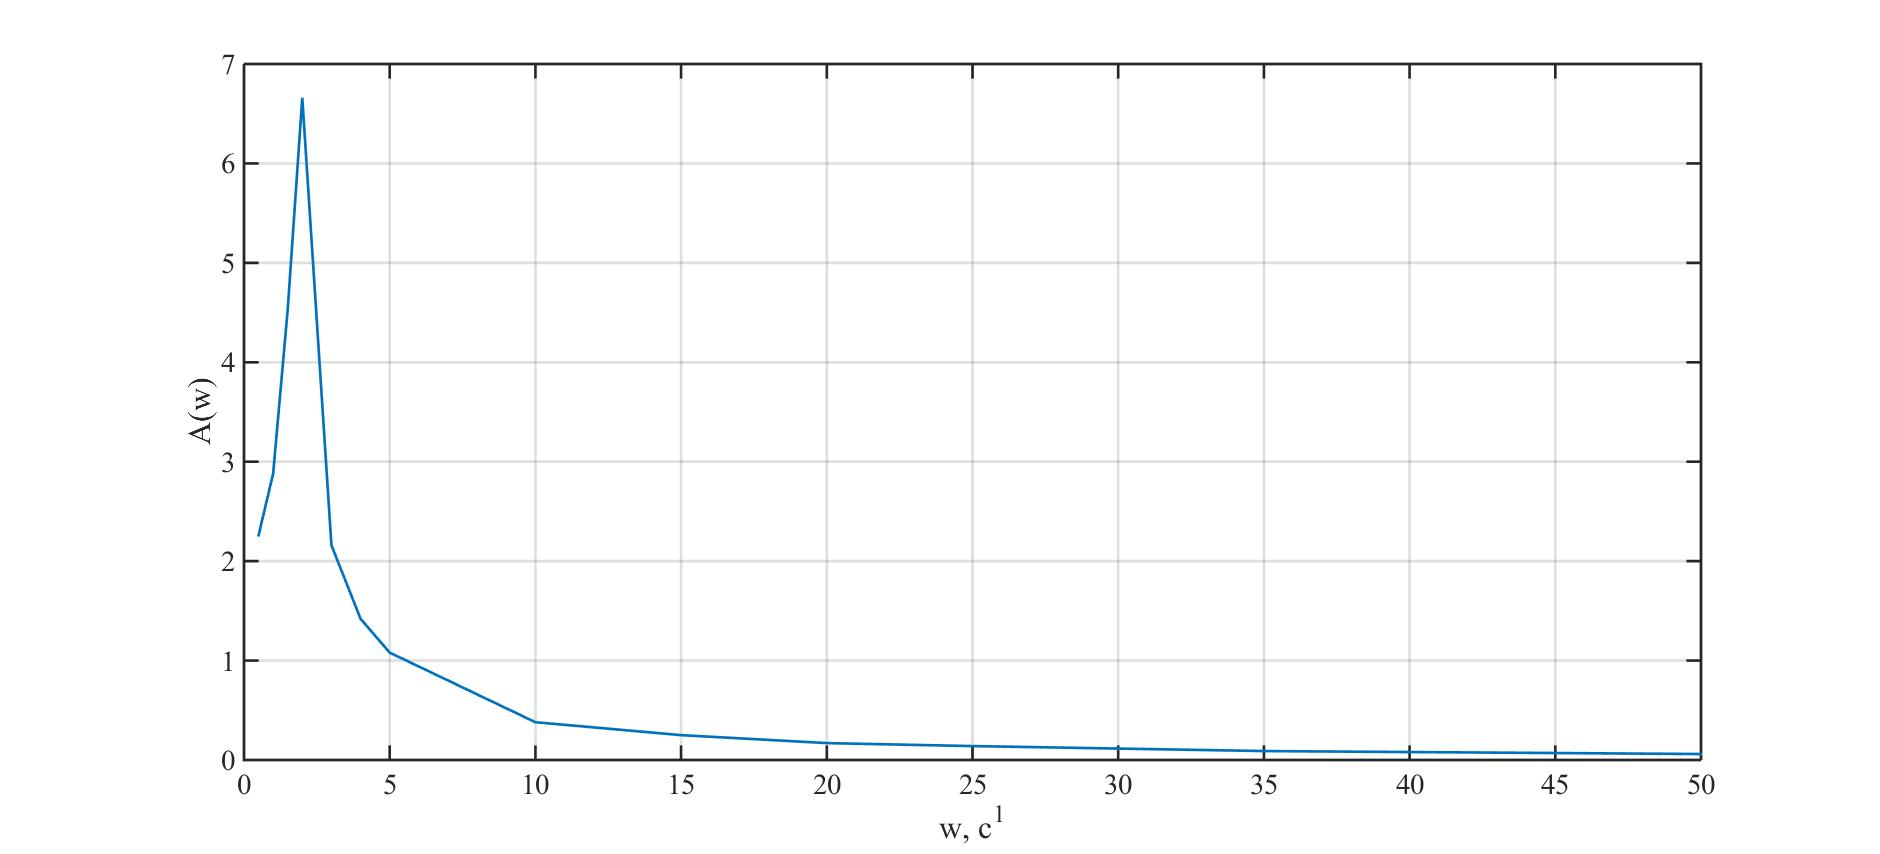
\includegraphics[width=1\linewidth]{1/aw}}
	\caption{АЧХ}
	\label{1achh}
\end{figure}


\begin{figure}[h!]
	\center{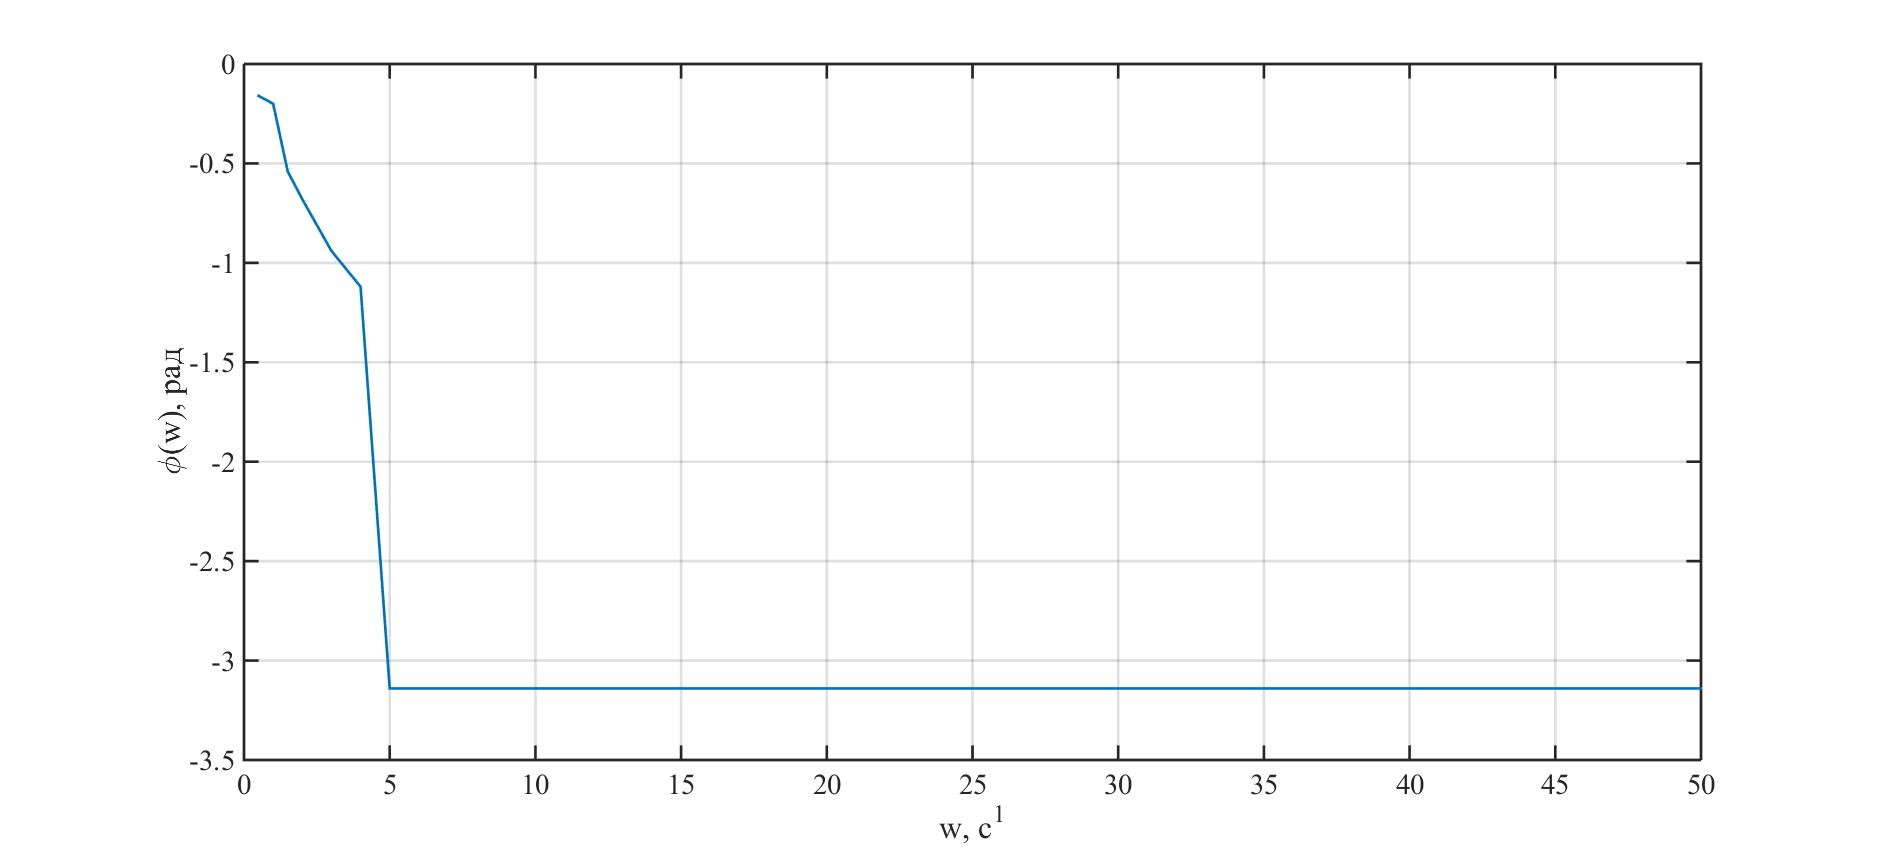
\includegraphics[width=1\linewidth]{1/fi}}
	\caption{ФЧХ}
	\label{1fchh}
\end{figure}

\newpage

\begin{figure}[h!]
	\center{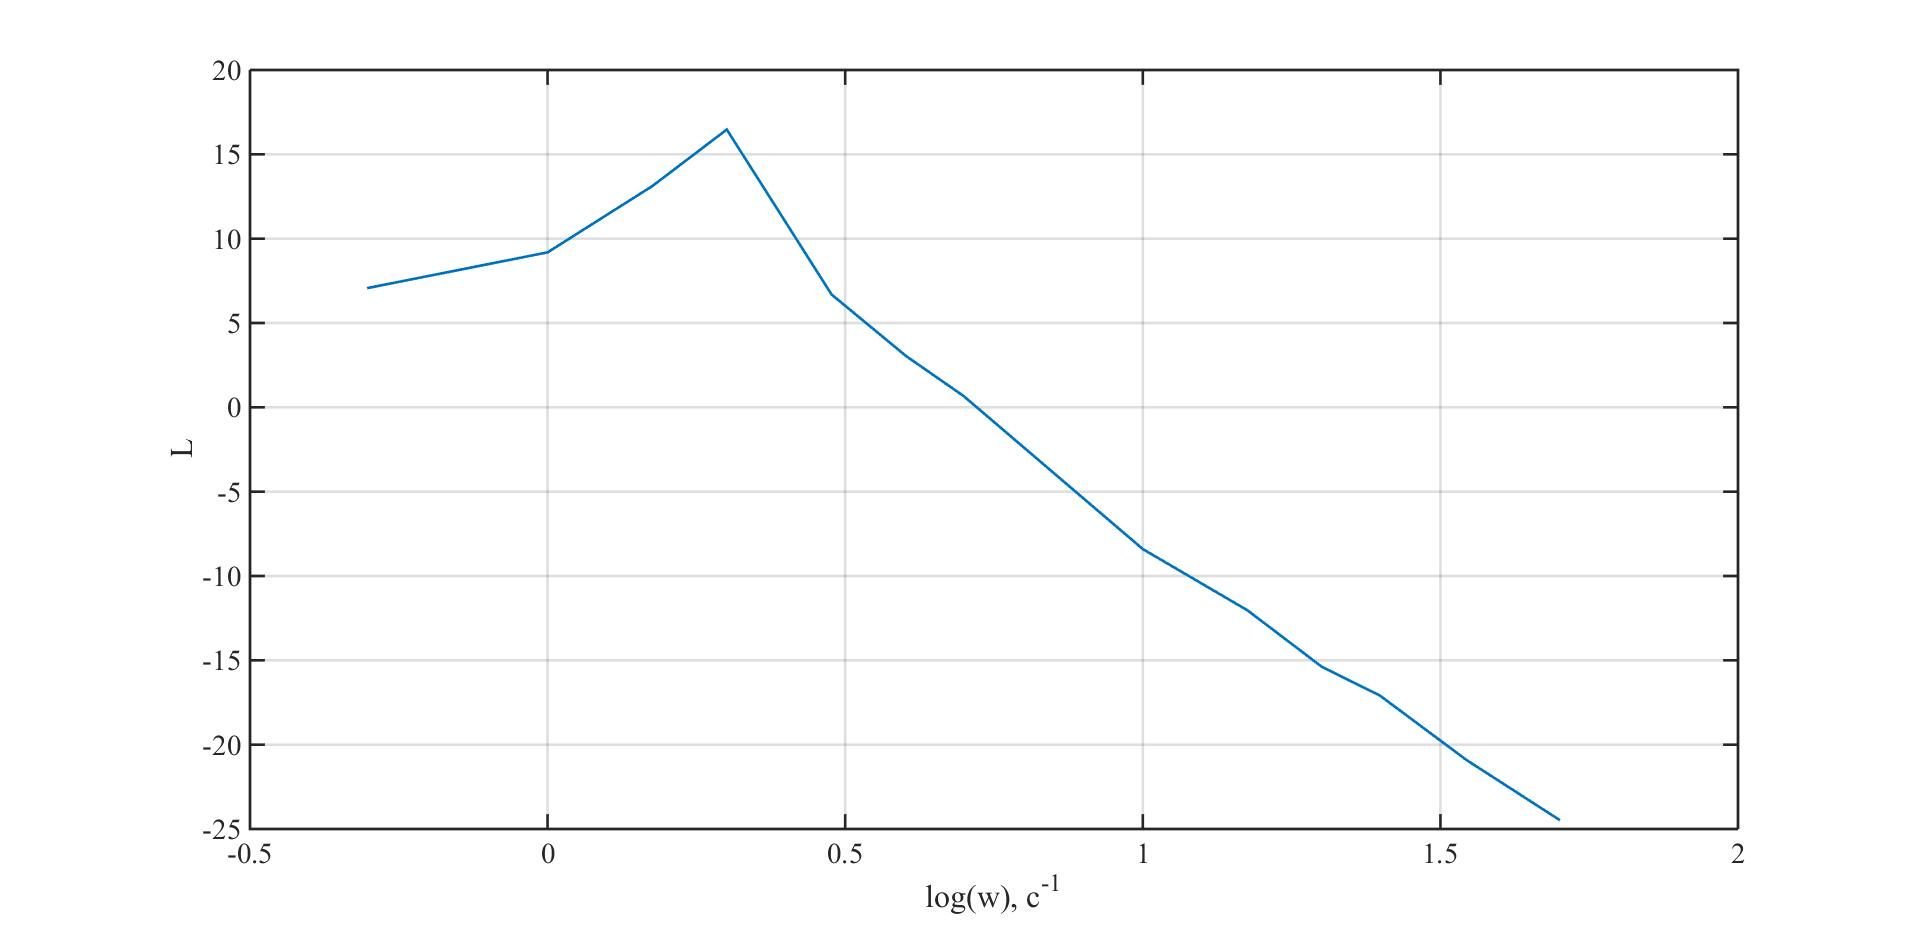
\includegraphics[width=1\linewidth]{1/Llgw}}
	\caption{ЛФЧХ}
	\label{1lfchh}
\end{figure}


\begin{figure}[h!]
	\center{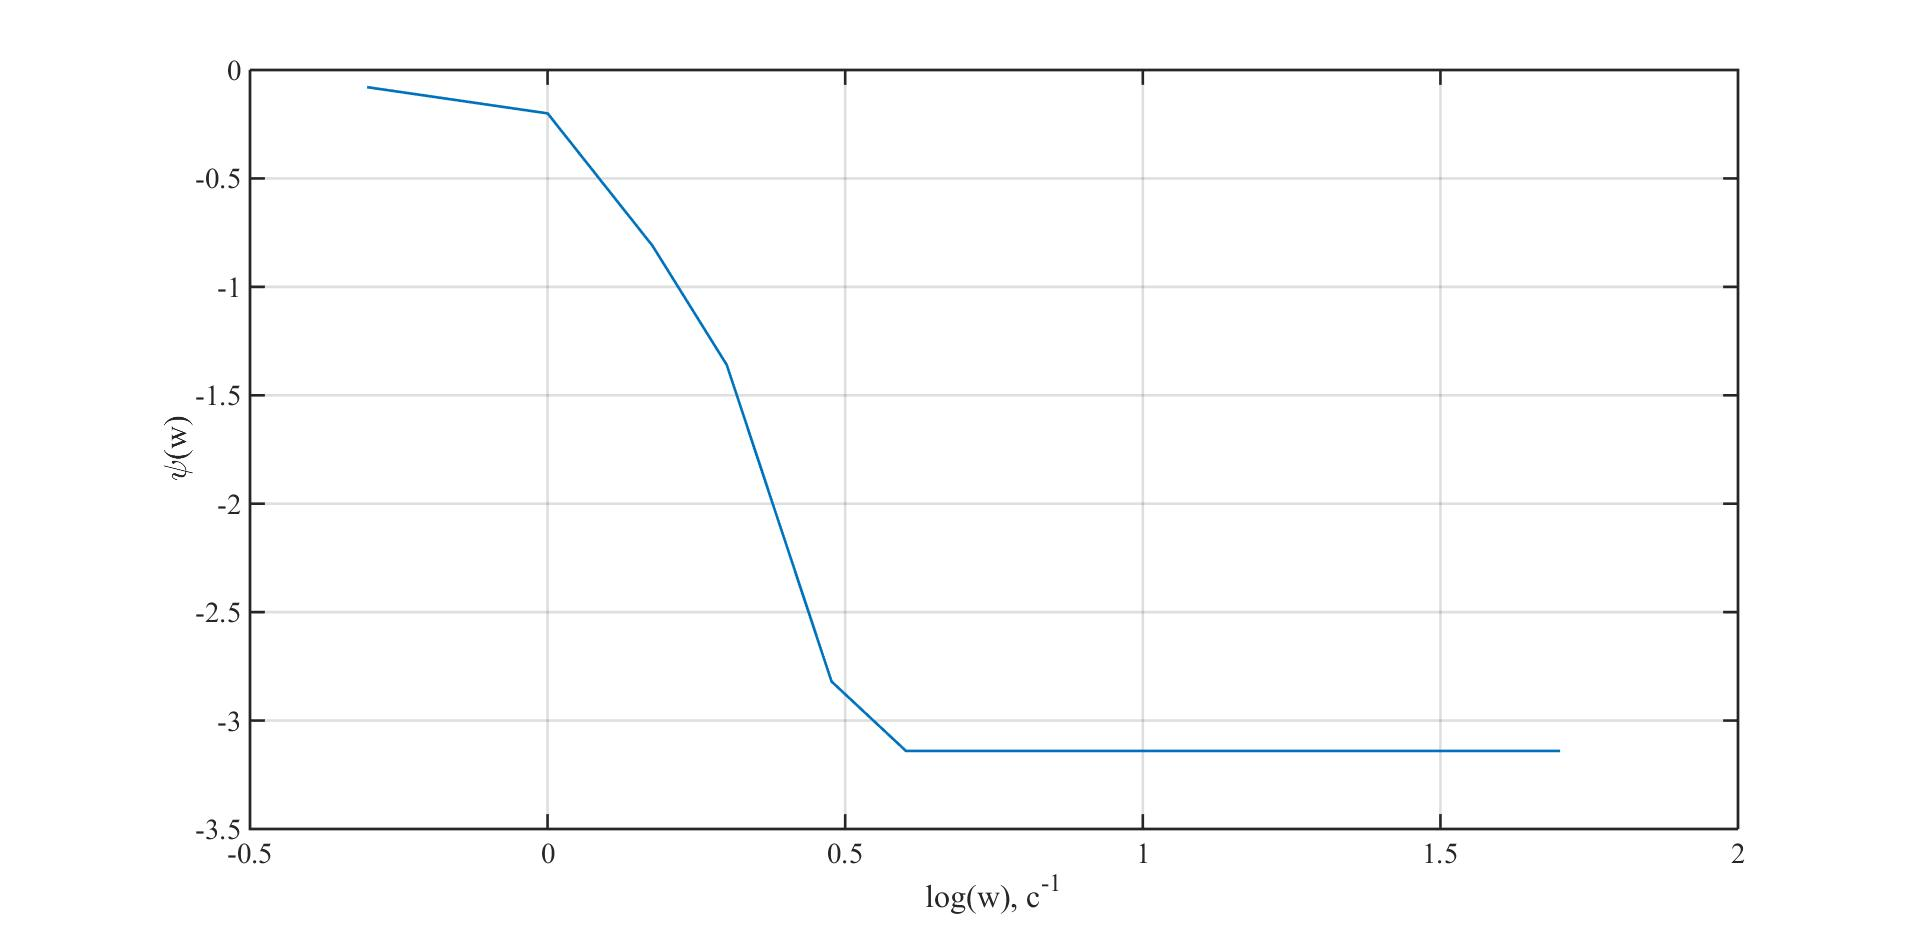
\includegraphics[width=1\linewidth]{1/psi}}
	\caption{ЛAЧХ}
	\label{1lachh}
\end{figure}

\newpage

\begin{figure}[h!]
	\center{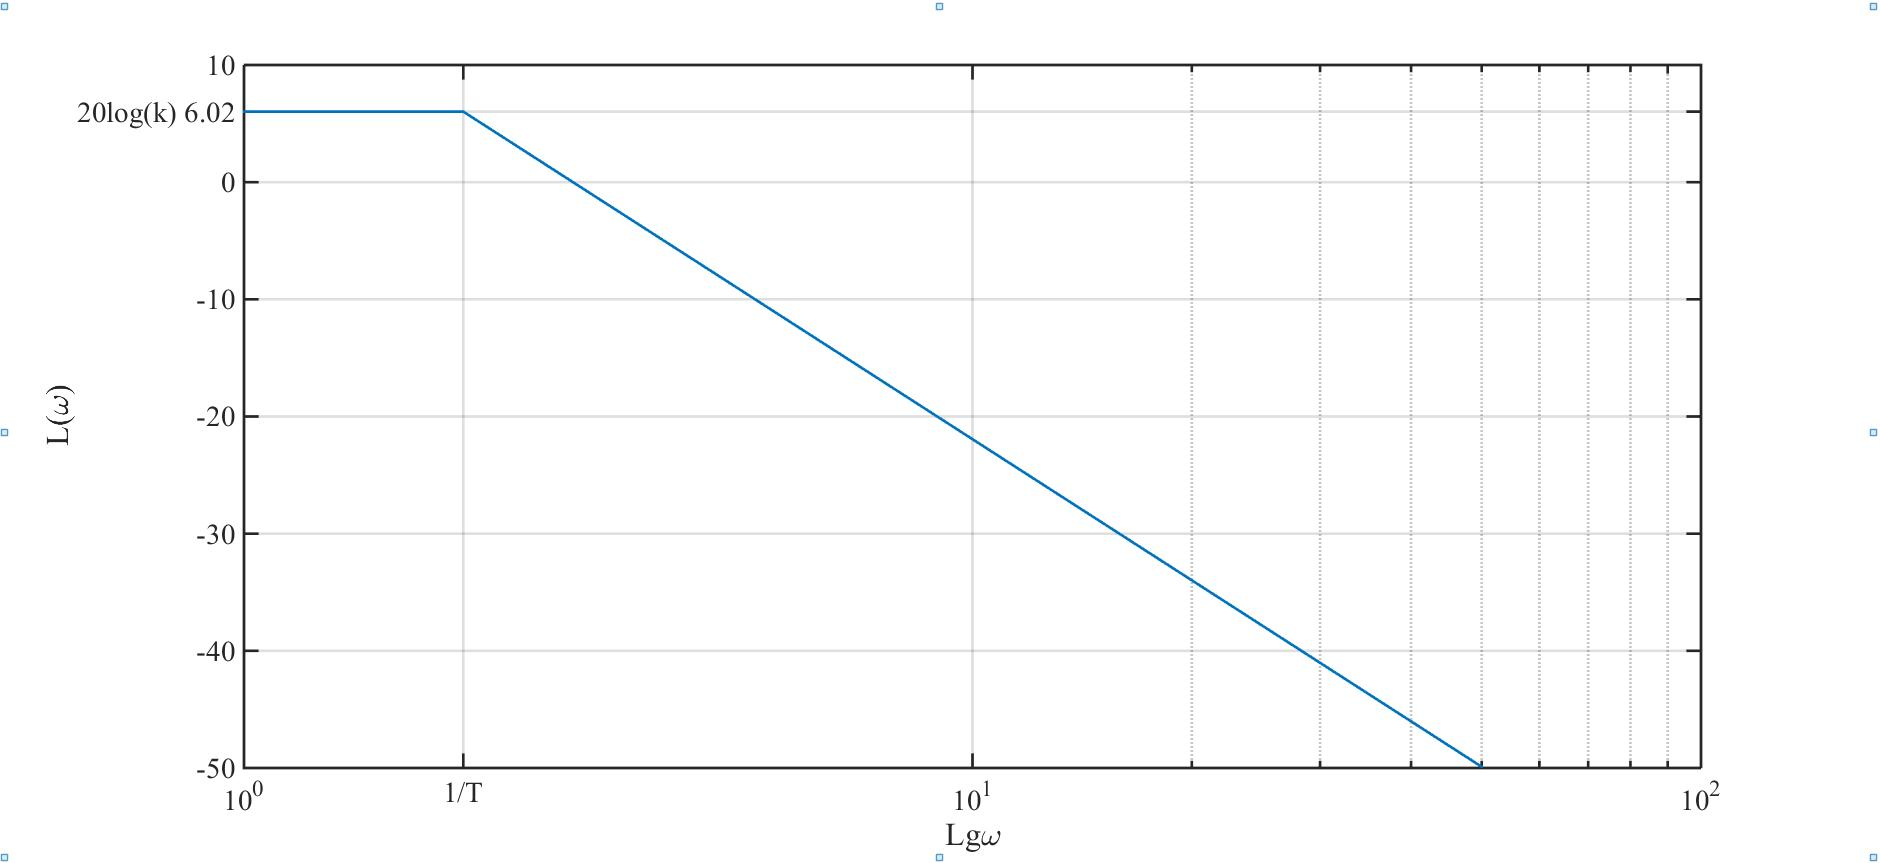
\includegraphics[width=1\linewidth]{1/lachxass}}
	\caption{Асимптотическая ЛAЧХ}
	\label{1alachh}
\end{figure}


\begin{figure}[h!]
	\center{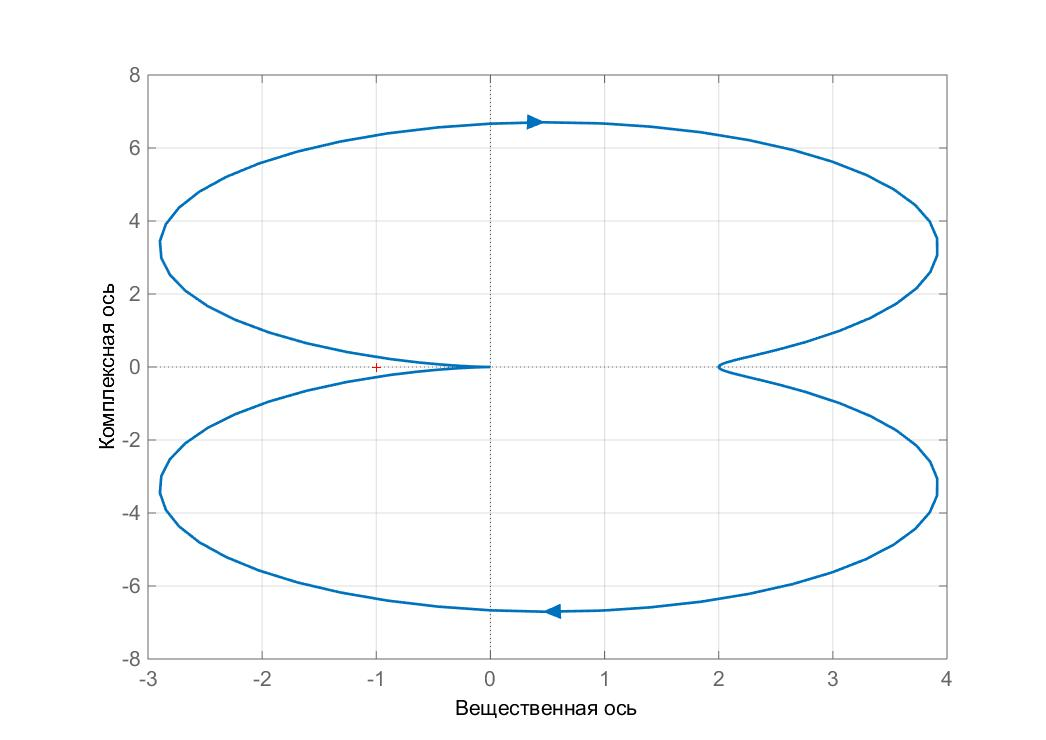
\includegraphics[width=1\linewidth]{1/afchx_2}}
	\caption{АФЧХ}
	\label{1afchh}
\end{figure}

\newpage
\begin{center}
	\section{Идеальное интегрирующее звено}
\end{center}\par
В таблице \ref{tab:integr} представлены экспериментальные данные идеального интегрирующего звена.

\begin{equation}
	L(\omega) = 20\lg(k)-20\lg(\omega)
\end{equation}

\begin{table}[h]
	\caption{Экспериментальные данные идеального интегрирующего звена}
	\label{tab:integr}
	\begin{tabular}{|c|c|c|c|c|}
		\hline
		$\omega$, рад/c   & $\lg(\omega)$   & $A(\omega)$ & $L(\omega)$   & $\psi(\omega)$, град   \\
		\hline
		0,5 & -0,30 & 8    & 18,06   & -3,16 \\
		\hline
		1   & 0,00  & 4    & 12,04   & -9,38 \\
		\hline
		1,5 & 0,18  & 2,66 & 8,49   & -3,18 \\
		\hline
		2   & 0,30  & 2    & 6,02    & -3,14 \\
		\hline
		3   & 0,48  & 1,33 & 2,47    & -3,12 \\
		\hline
		4   & 0,60  & 1    & 0              & -3,12 \\
		\hline
		5   & 0,70  & 0,8  & -1,93    & -3,1  \\
		\hline
		10  & 1,00  & 0,4  & -7,95   & -3,1  \\
		\hline
		15  & 1,18  & 0,26 & -11,70   & -3,15 \\
		\hline
		20  & 1,30  & 0,2  & -13,97   & -3    \\
		\hline
		25  & 1,40  & 0,16 & -15,91   & -3    \\
		\hline
		35  & 1,54  & 0,11 & -19,17    & -3,15 \\
		\hline
		50  & 1,70  & 0,08 & -21,93   & -3   \\
		\hline
	\end{tabular}
\end{table}

На рисунках \ref{2achh}-\ref{2afchh} представлены частотные и логарифмические характеристики идеального интегрирующего звена.

\newpage

\begin{figure}[h!]
	\center{\includegraphics[width=1\linewidth]{2/aw2}}
	\caption{АЧХ}
	\label{2achh}
\end{figure}
\begin{figure}[h!]
	\center{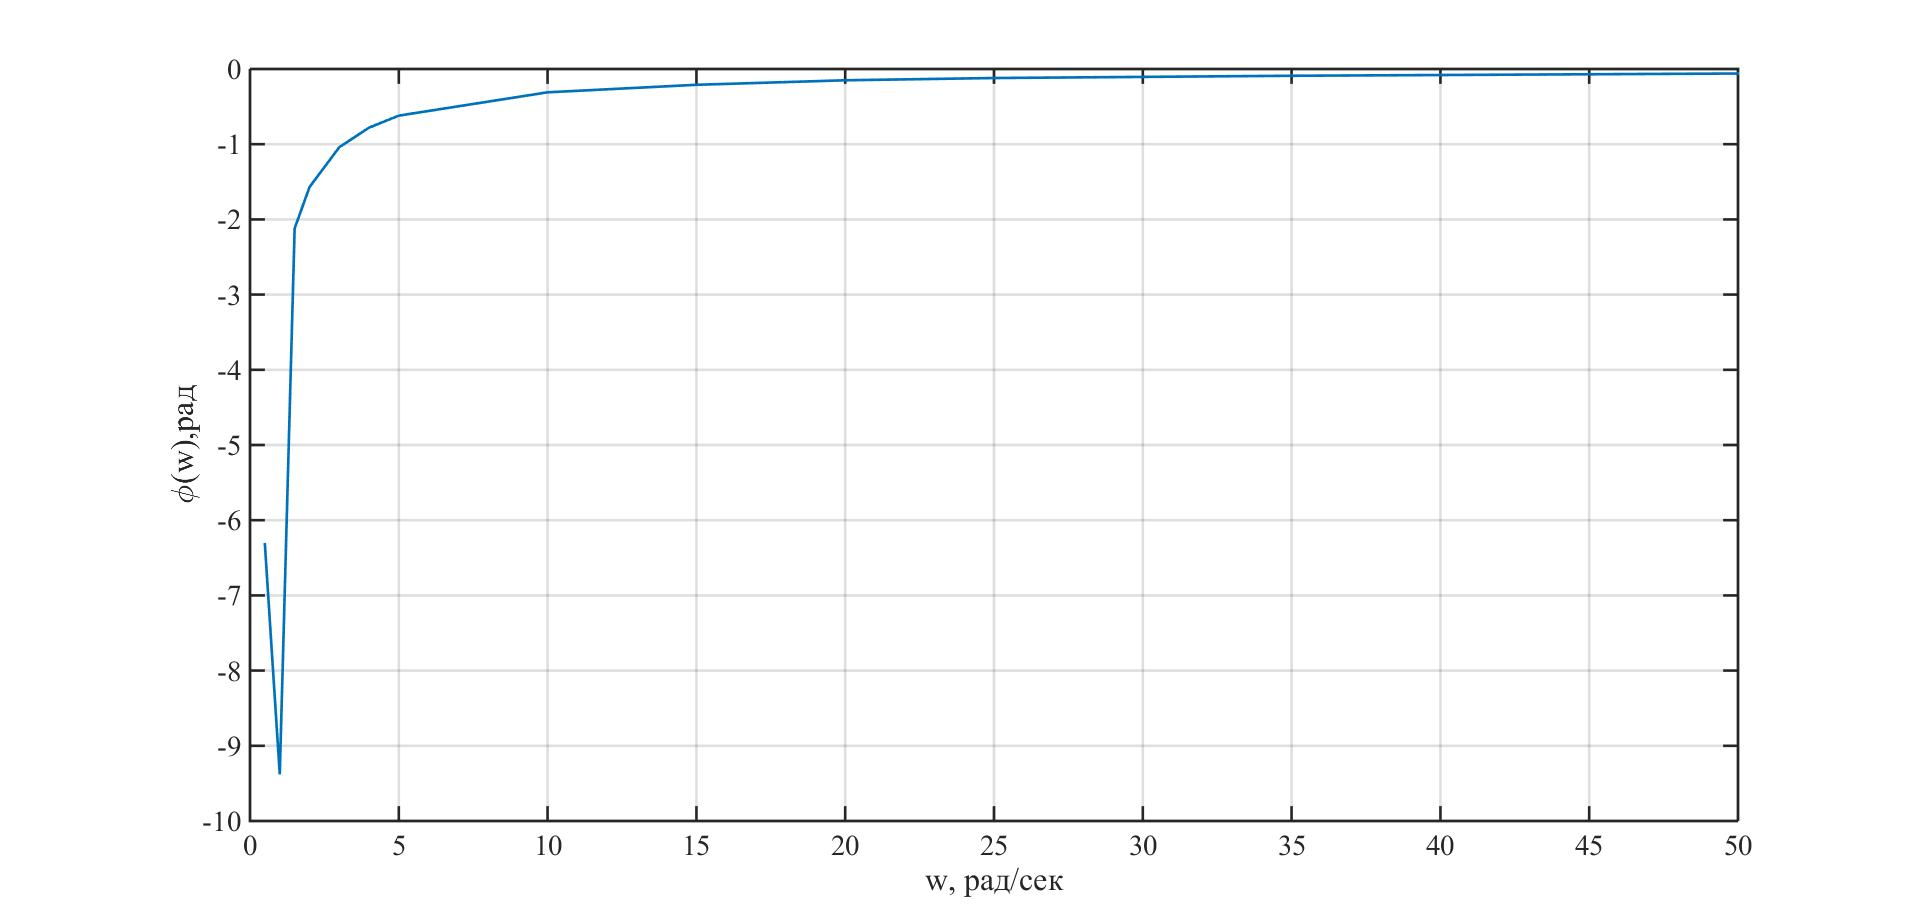
\includegraphics[width=1\linewidth]{2/fi2}}
	\caption{ФЧХ}
	\label{2fchh}
\end{figure}

\newpage

\begin{figure}[h!]
	\center{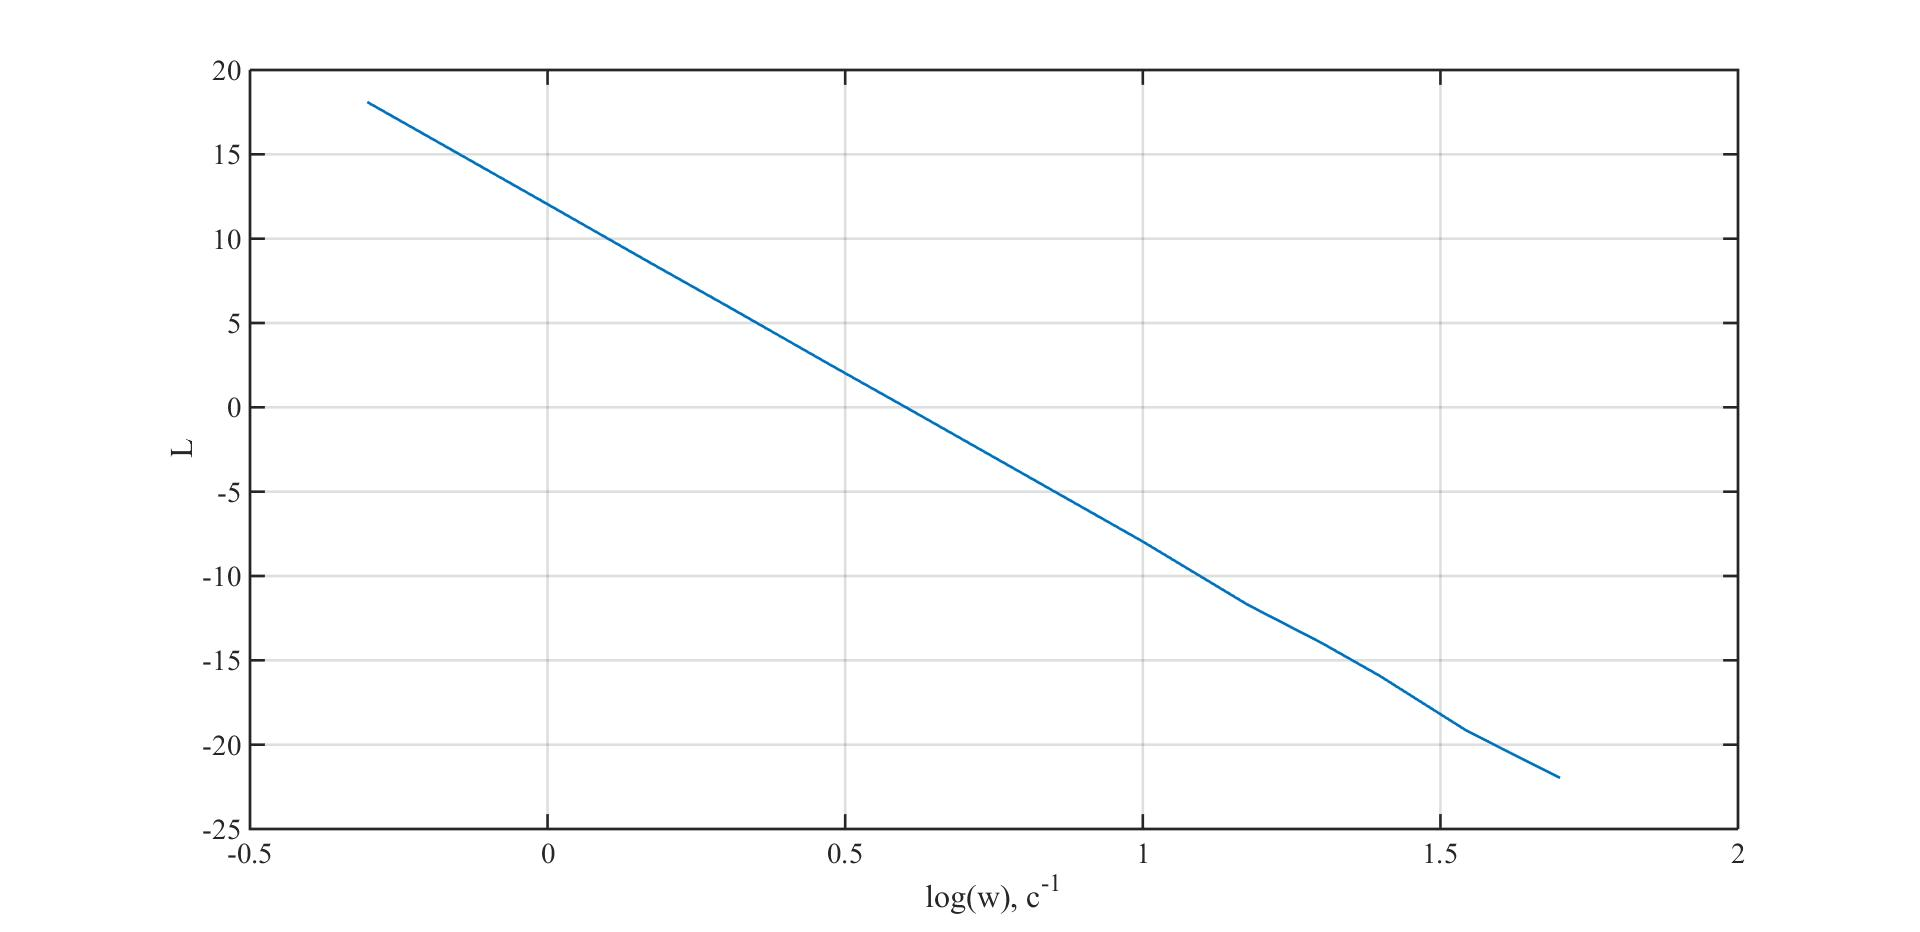
\includegraphics[width=1\linewidth]{2/Llgw2}}
	\caption{ЛФЧХ}
	\label{2lfchh}
\end{figure}
\begin{figure}[h!]
	\center{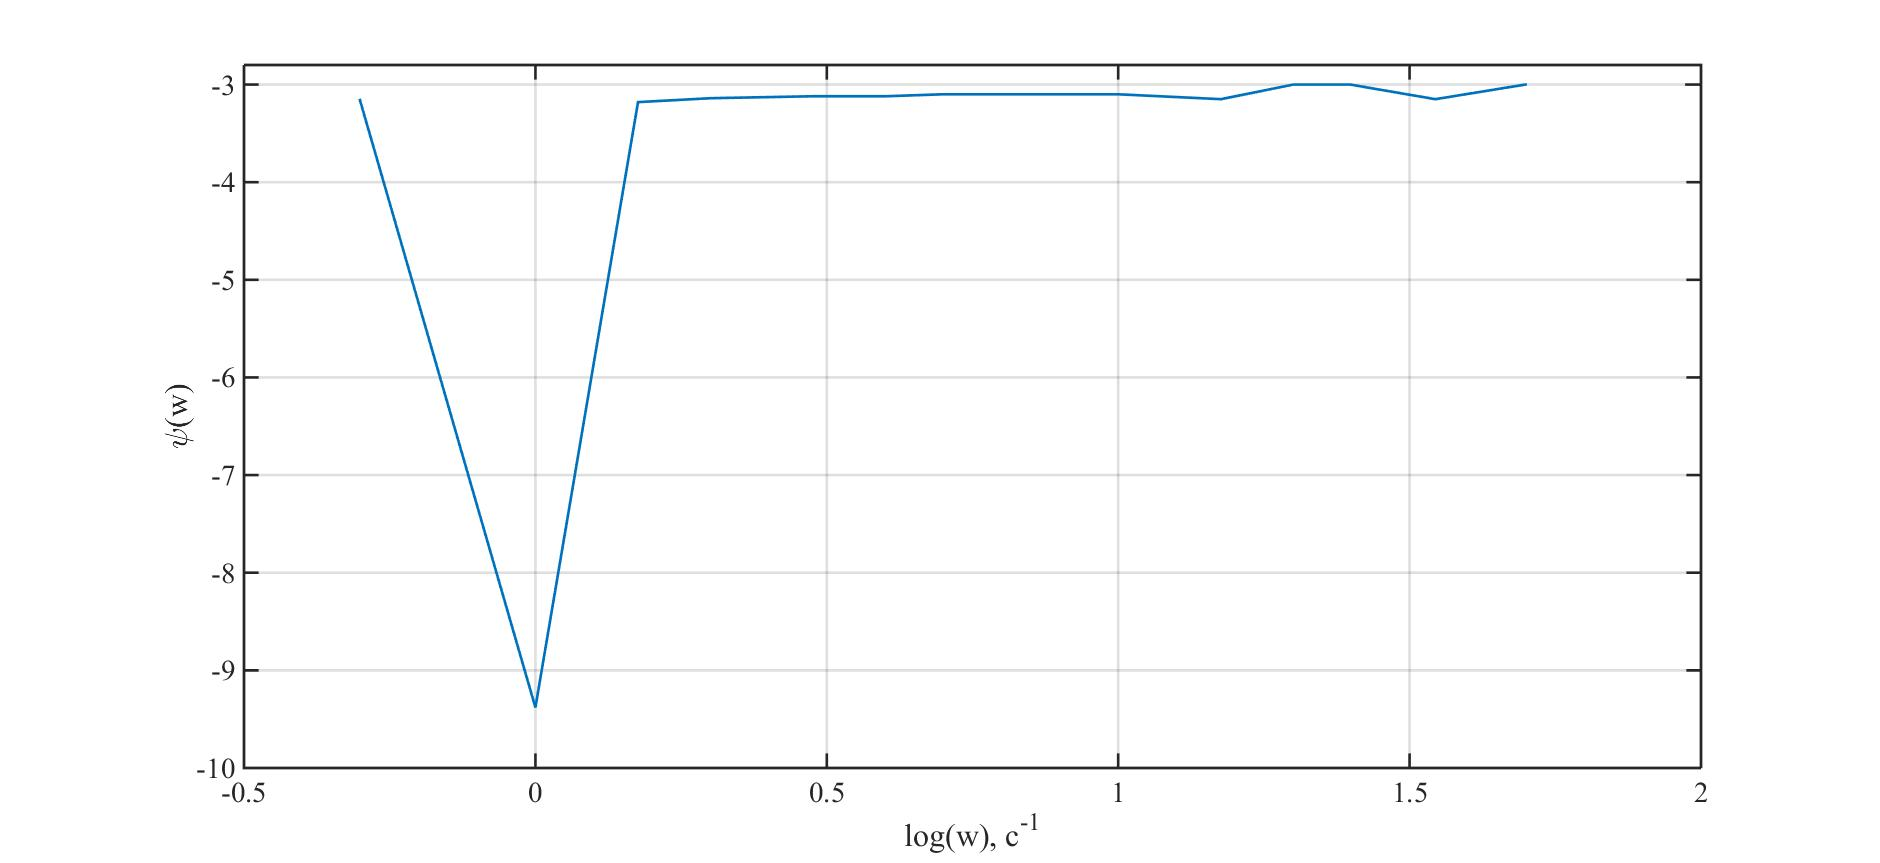
\includegraphics[width=1\linewidth]{2/psi2}}
	\caption{ЛAЧХ}
	\label{2lachh}
\end{figure}

\newpage

\begin{figure}[h!]
	\center{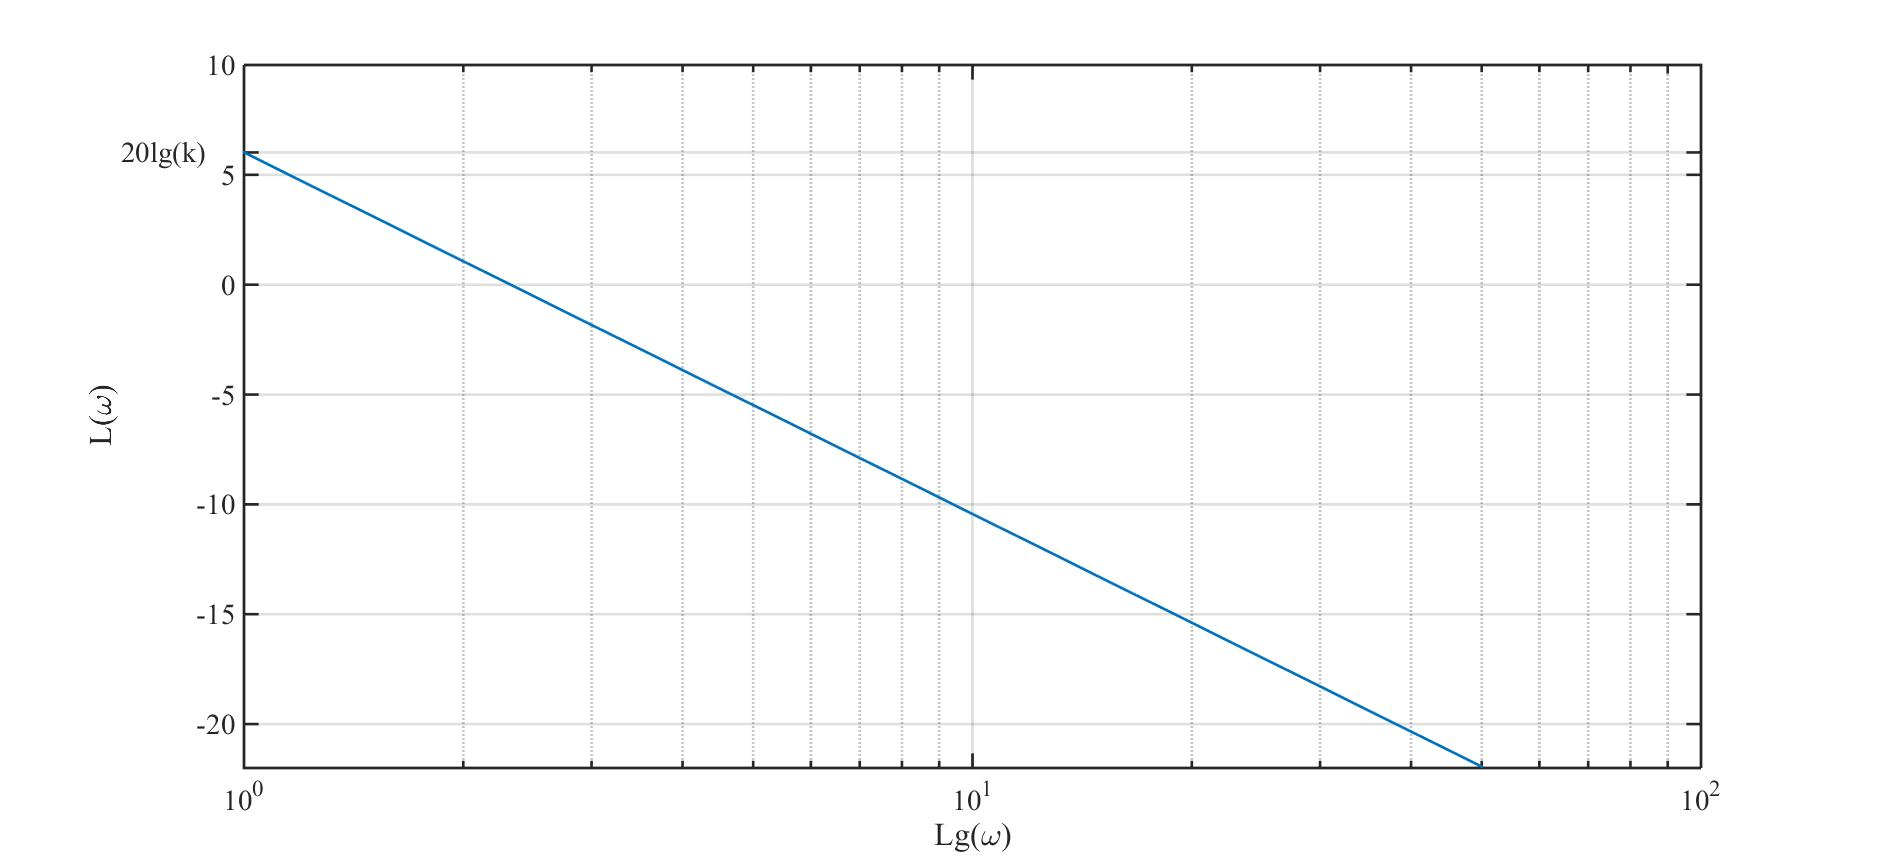
\includegraphics[width=1\linewidth]{2/lachxass2}}
	\caption{Асимптотическая ЛAЧХ}
	\label{2alachh}
\end{figure}
\begin{figure}[h!]
	\center{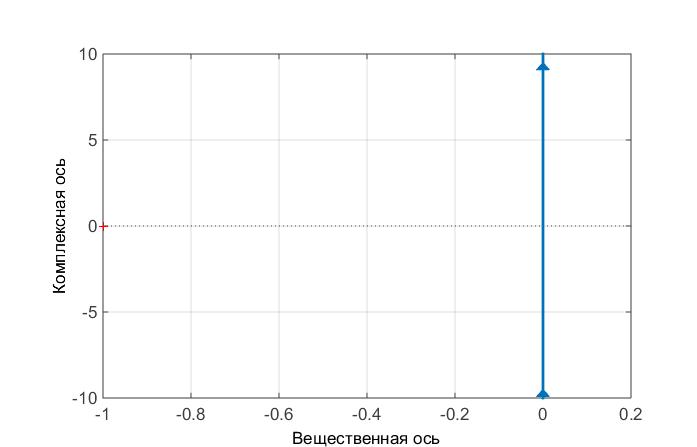
\includegraphics[width=1\linewidth]{2/afchx2_1}}
	\caption{АФЧХ}
	\label{2afchh}
\end{figure}

\newpage
\begin{center}
	\section{Изодромное звено}
\end{center}\par
В таблице \ref{tab:izodr} представлены экспериментальные данные изодромного звена.
Уравнение асимптотической ЛАЧХ
\begin{equation}
	L(\omega)=20\lg(k)-20\lg(\omega)+20\lg\sqrt{1+\omega^2*T^2}
\end{equation}

\begin{table}[h]
	\caption{Экспериментальные данные изодромного звена}
	\label{tab:izodr}
	\begin{tabular}{|c|c|c|c|c|}
		\hline
		$\omega$, рад/c   & $\lg(\omega)$   & $A(\omega)$ & $L(\omega)$    & $\psi(\omega)$, град   \\
		\hline
		0,5 & -0,30 & 4,82 & 13,66     & -1,57  \\
		\hline
		1   & 0,00  & 3,23 & 10,18     & -0,92  \\
		\hline
		1,5 & 0,18  & 2,77 & 8,84     & -0,63  \\
		\hline
		2   & 0,30  & 2,56 & 8,16     & -0,48  \\
		\hline
		3   & 0,48  & 2,36 & 7,45     & -0,33  \\
		\hline
		4   & 0,60  & 2,26 & 7,08     & -0,24  \\
		\hline
		5   & 0,70  & 2,21 & 6,88     & -0,2   \\
		\hline
		10  & 1,00  & 2,1  & 6,44     & -0,1   \\
		\hline
		15  & 1,18  & 2,06 & 6,27    & -0,06  \\
		\hline
		20  & 1,30  & 2,05 & 6,23    & -0,04  \\
		\hline
		25  & 1,40  & 2,04 & 6,19    & -0,05  \\
		\hline
		35  & 1,54  & 2,02 & 6,10    & -0,035 \\
		\hline
		50  & 1,70  & 2,02 & 6,10    & 0     \\
		\hline
	\end{tabular}
\end{table}

На рисунках \ref{3achh}-\ref{3afchh} представлены частотные и логарифмические характеристики изодромного звена.

\newpage

\begin{figure}[h!]
	\center{\includegraphics[width=1\linewidth]{3/aw3}}
	\caption{АЧХ}
	\label{3achh}
\end{figure}
\begin{figure}[h!]
	\center{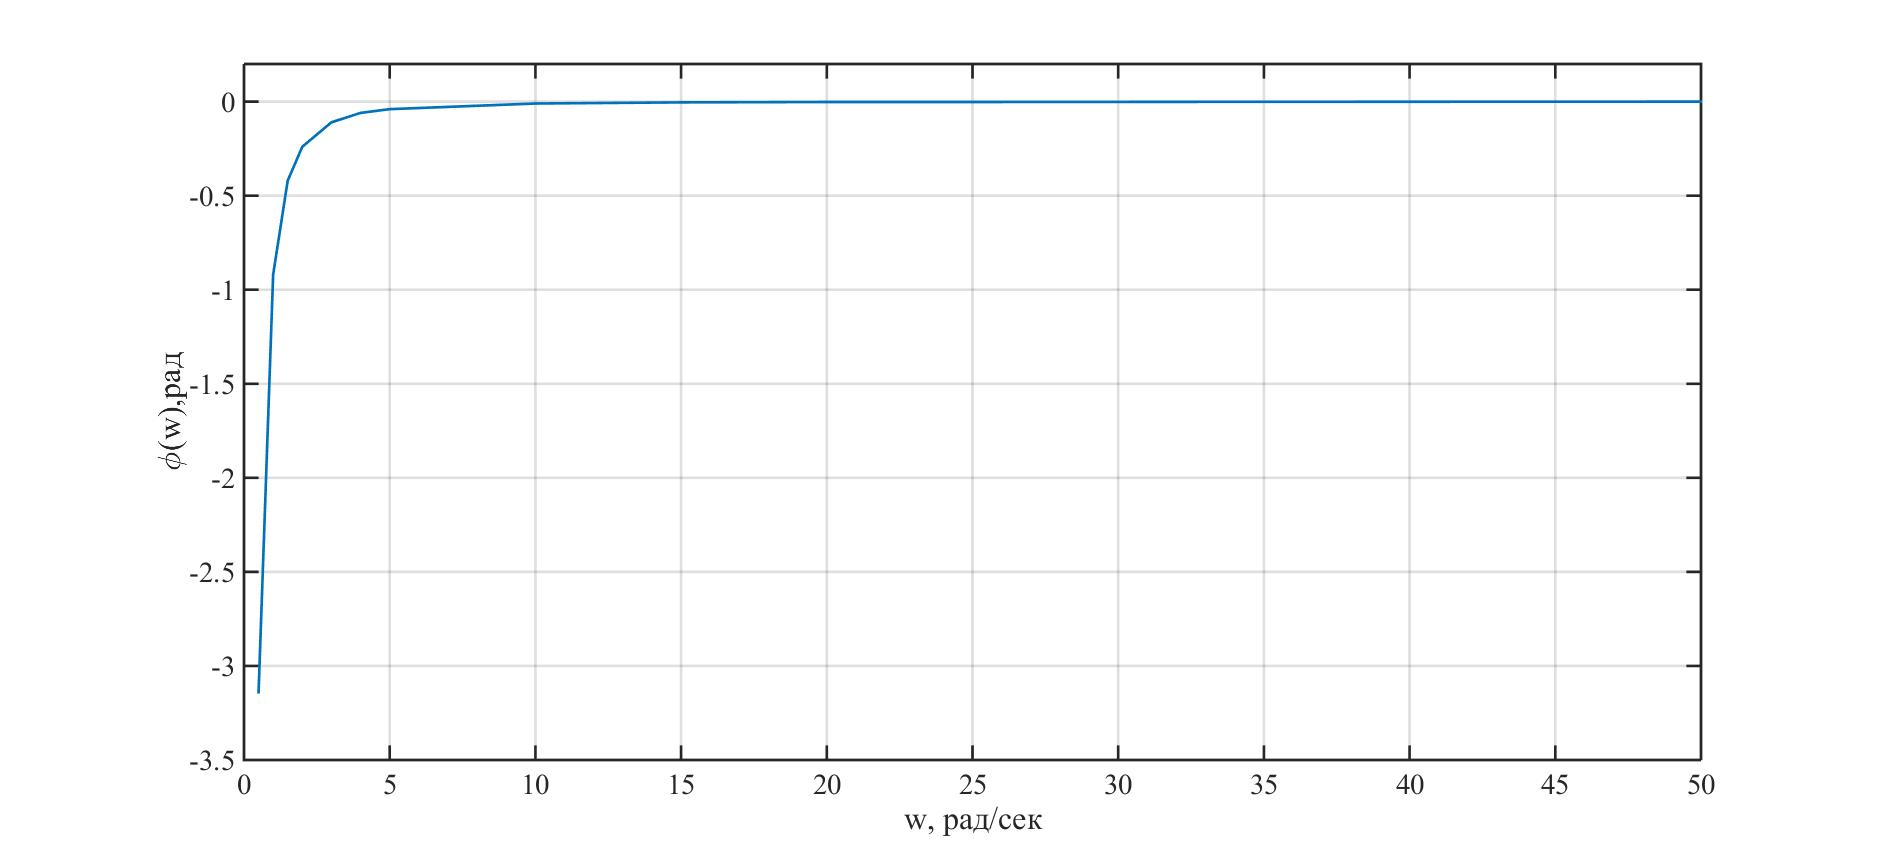
\includegraphics[width=1\linewidth]{3/fi3}}
	\caption{ФЧХ}
	\label{3fchh}
\end{figure}

\newpage

\begin{figure}[h!]
	\center{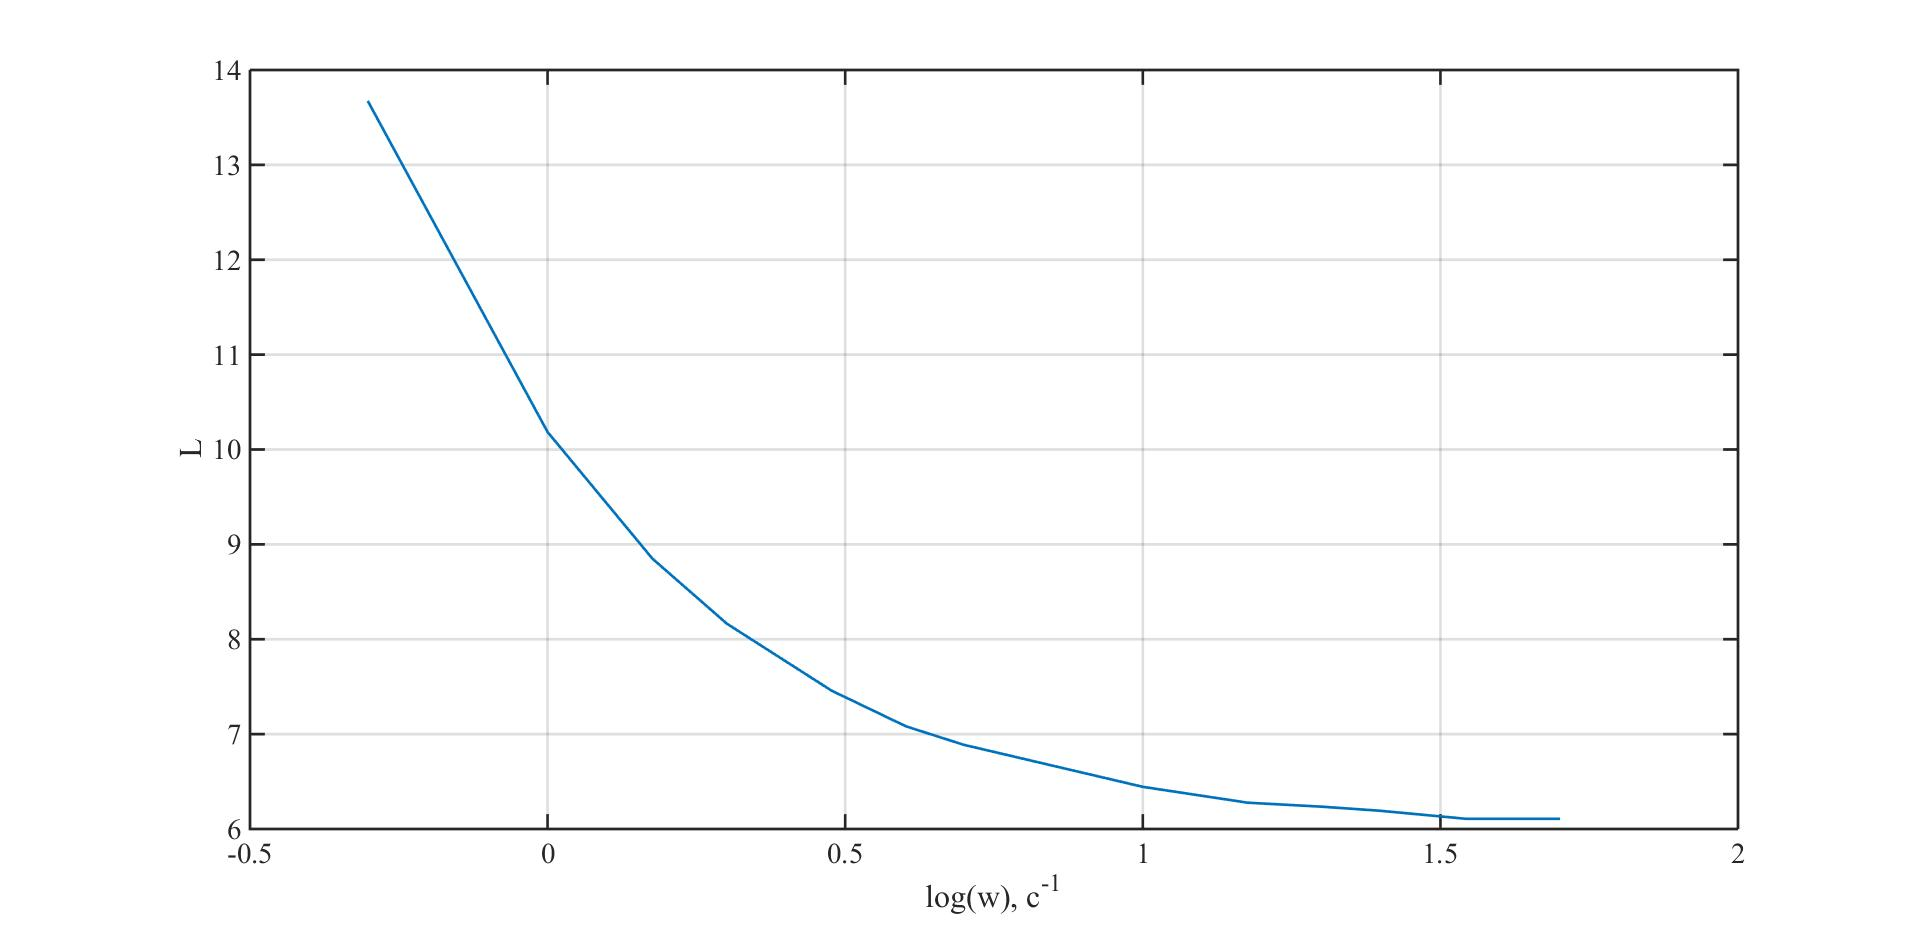
\includegraphics[width=1\linewidth]{3/Llgw3}}
	\caption{ЛФЧХ}
	\label{3lfchh}
\end{figure}
\begin{figure}[h!]
	\center{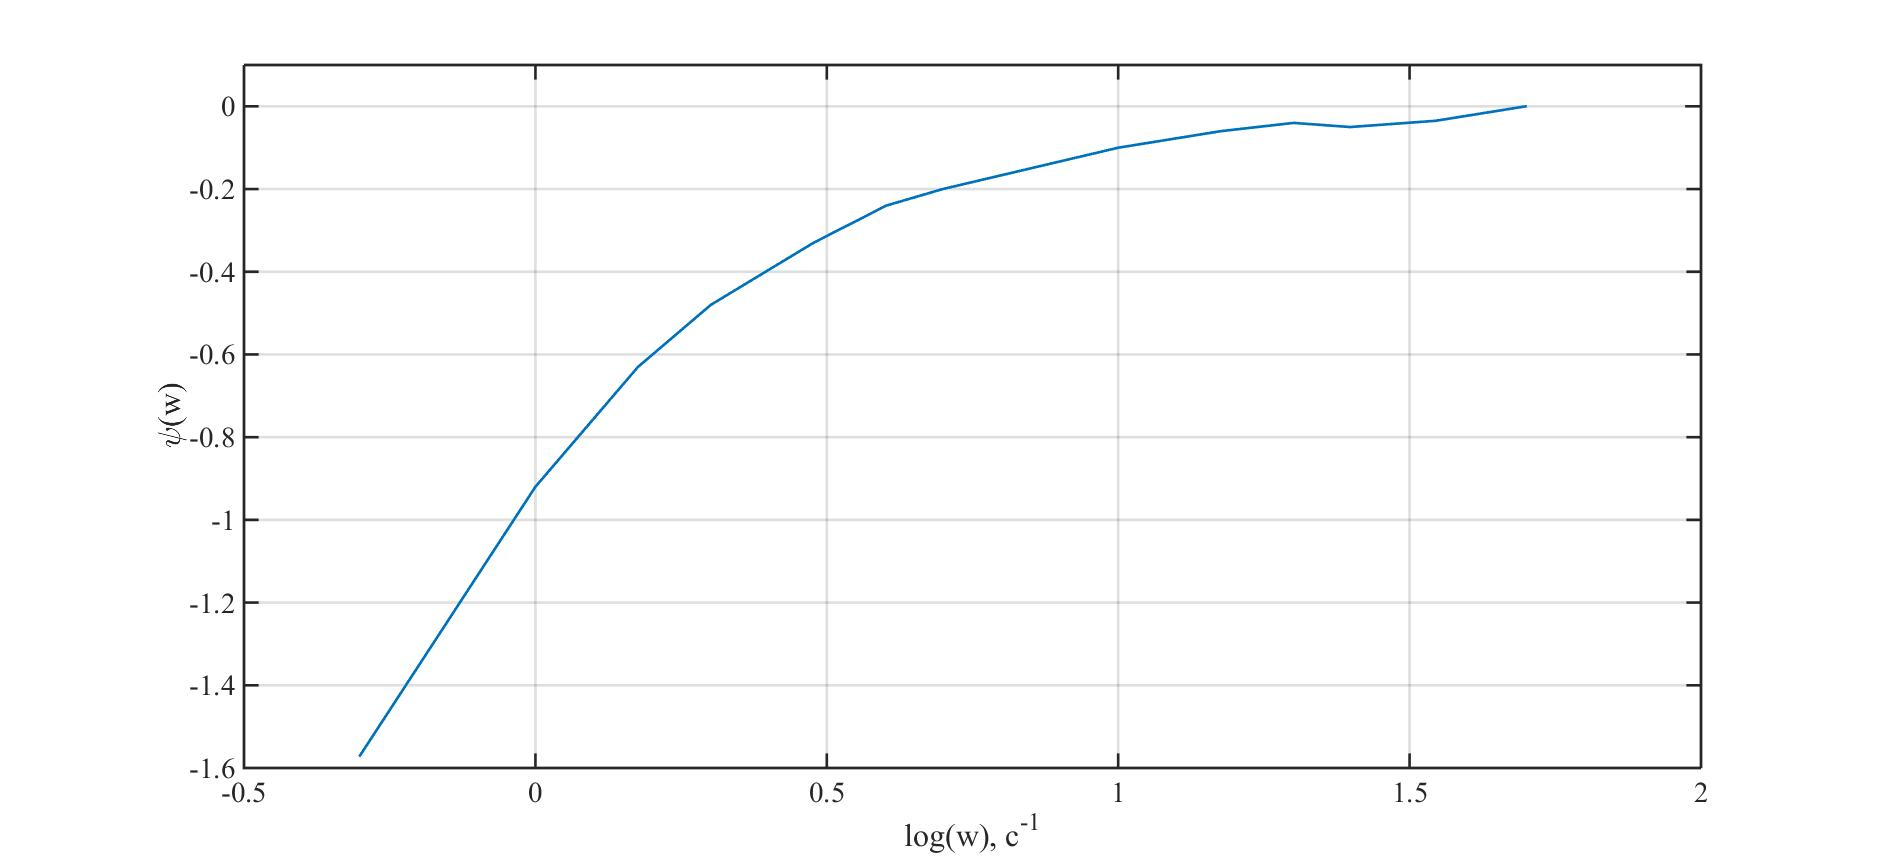
\includegraphics[width=1\linewidth]{3/psi3}}
	\caption{ЛAЧХ}
	\label{3lachh}
\end{figure}

\newpage

\begin{figure}[h!]
	\center{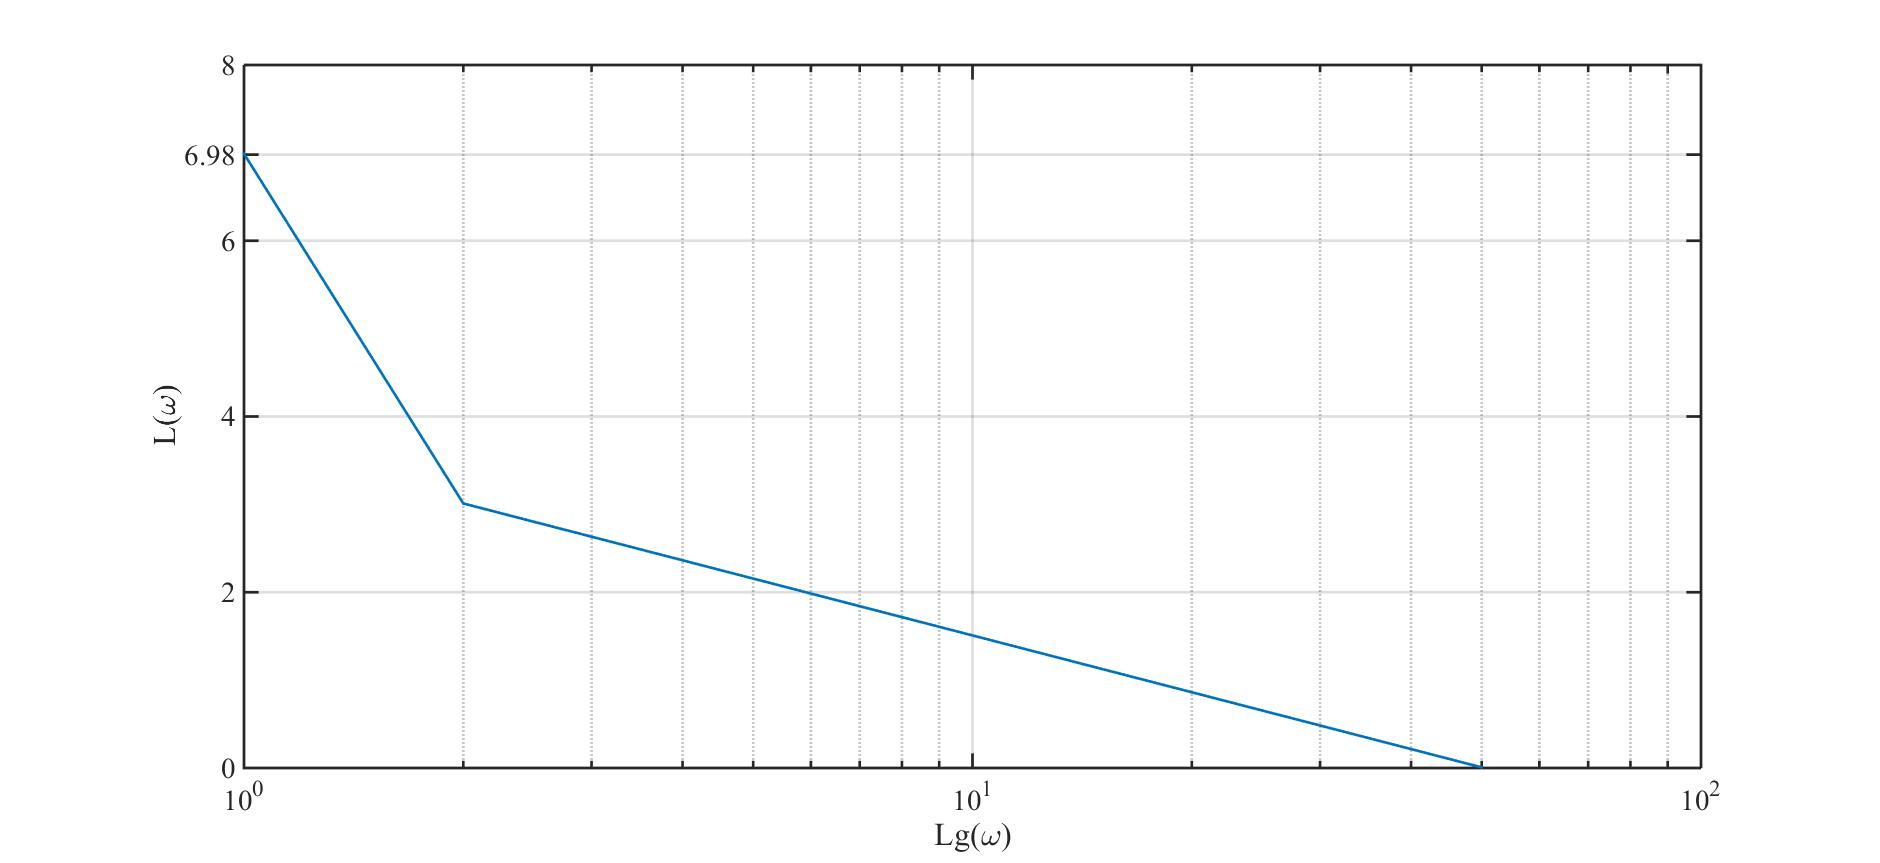
\includegraphics[width=1\linewidth]{3/lachxass3}}
	\caption{Асимптотическая ЛAЧХ}
	\label{3alachh}
\end{figure}
\begin{figure}[h!]
	\center{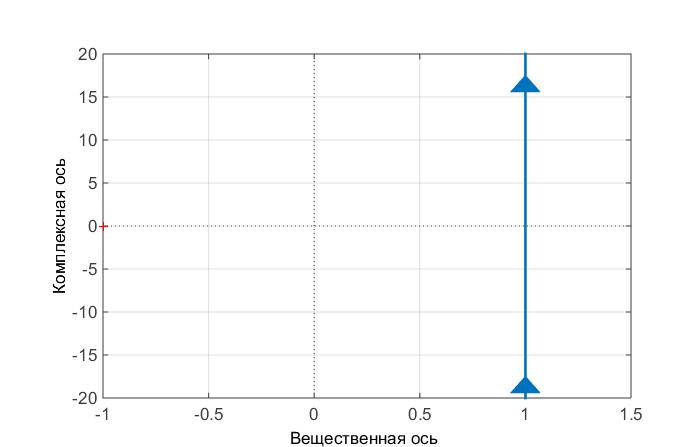
\includegraphics[width=1\linewidth]{3/afchx3_1}}
	\caption{АФЧХ}
	\label{3afchh}
\end{figure}

\newpage

\begin{center}
	\section*{Вывод}
\end{center}\par
В данной лабораторной работе были исследованы частотные обычные и логарифмические характеристики трех типовых звеньев: колебательного, идеального интегрирующего и изодромного. В ходе лабораторной работы было выявлено, что асимптотические ЛАЧХ сходятся построенными по математическим моделям графиками.

\end{document}